\documentclass[]{beamer} % Use the beamer class for presentations, 'handout' option to suppress \pause

\input{Lecture-Slides/preamble.txt}

\usepackage{animate} % Animations

% Packages for math and plots
\usepackage{amsmath}
\usepackage{graphicx}
\usepackage{booktabs}

\usepackage{pgfplots}
% Nice color sets, see see http://colorbrewer2.org/
\usepgfplotslibrary{colorbrewer}
% initialize Set1-4 from colorbrewer (we're comparing 4 classes),
\pgfplotsset{compat = 1.18, cycle list/Set1-8}
% Tikz is loaded automatically by pgfplots
\usetikzlibrary{pgfplots.statistics, pgfplots.colorbrewer}
% provides \pgfplotstabletranspose
\usepackage{pgfplotstable}

% Title and Author Info

\title{Introduction to Statistical Methods in Political Science}
\subtitle{Lecture Notes: Simulations of Random Events and Probability}
\author{Ignacio Urbina \texorpdfstring{\\ \vspace{0.3em}}{ } \scriptsize \textcolor{gray}{Ph.D. Candidate in Political Science}}

\date{}


\begin{document}

% Title slide
\begin{frame}
    \titlepage
\end{frame}

\begin{frame}{Problem Setup}
  \begin{columns}[T] % Align content at the top
    \column{0.6\textwidth}
      \begin{itemize}
        \item Suppose we conducted an experiment flipping a coin 10 times.
        \item Observed result: 6 heads, 4 tails. \emph{Does this data suggest the coin is biased?}
        \item \textbf{Goal: Determine if this suggests the coin is biased.}
        \item Approach: Simulate fair coin flips and compare.
      \end{itemize}
    \column{0.4\textwidth}
    \vspace{3.5em}
      \centering
      \animategraphics[loop, autoplay, width=\textwidth, trim=10 50 175 50, clip]{10}{Images/Coin-Anim/frame-}{000}{009}
  \end{columns}
\end{frame}


% Statistical Simulation Concept
\begin{frame}{Statistical Simulation Concept}
    \begin{center}

    \makebox[\textwidth]{ % Expands the box to the full width
        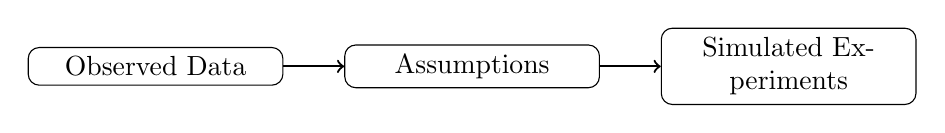
\begin{tikzpicture}[node distance=0.02cm, every node/.style={draw, text width=3cm, align=center, rounded corners}]
            \node (data) {Observed Data};
            \node (assumptions) [right of=data, xshift=4cm] {Assumptions};
            \node (experiments) [right of=assumptions, xshift=4cm] {Simulated Experiments};

            \draw[->, thick] (data) -- (assumptions);
            \draw[->, thick] (assumptions) -- (experiments);
        \end{tikzpicture}
    }

    \end{center}
    \begin{itemize}
        \item Data: We observe real-world coin flips.
        \item Assumptions: Assume the coin is fair with $P(H) = 0.5$.
        \item Experiments: Simulate many trials under these assumptions.
    \end{itemize}
\end{frame}

%%%%%%%%%
\begin{frame}{Where Do Random Numbers Come From?}
    \begin{itemize}
        \item Computers simulate randomness using \textbf{pseudo-random number generators (PRNGs)}.
        \item A PRNG is a deterministic algorithm that starts from a \textbf{seed value}.
        \item The \textbf{seed} is often based on the computer’s clock — for example:
            \begin{itemize}
                \item The number of milliseconds since the computer was turned on.
            \end{itemize}
        \item This makes the output different every time the program runs.
        \item Once seeded, the PRNG produces a sequence of numbers between 0 and 1 that appear random:
\[
                \texttt{random()} \rightarrow 0.732,\ 0.126,\ 0.984,\ \ldots
\]
        \item These values are not truly random, but they are \textit{random enough} for most statistical simulations.
    \end{itemize}
\end{frame}

%%%%%%%%%%
\begin{frame}{Using Random Numbers to Simulate Probabilities}
    \begin{itemize}
        \item We can use PRNG outputs to simulate real-world random events.
        \item Example: \textbf{Simulating a coin flip}.
            \begin{itemize}
                \item Generate a random number between 0 and 1.
                \item If the number is $< 0.5$, call it Heads; otherwise, Tails.
            \end{itemize}
        \item Why this works: Half the interval [0, 1] is below 0.5 $\Rightarrow$ $P(\text{Heads}) = 0.5$.
        \item To simulate a different probability (e.g., $P(\text{Success}) = 0.3$):
            \begin{itemize}
                \item Return success if the number is $< 0.3$.
            \end{itemize}
        \item This logic is the foundation of statistical simulations!
    \end{itemize}
\end{frame}



% Simulation
\begin{frame}{Simulation Approach}
    \begin{itemize}
        \item Assume a fair coin: $P(H) = 0.5$.
        \item Simulate 1,000 samples of 10 coin flips.
        \item Compute the proportion of heads in each sample.
        \item Estimate probability of getting $\geq 60\%$ heads.
    \end{itemize}
\end{frame}


\begin{frame}
    \frametitle{Distribution of Simulation Outcomes}

    \begin{figure}
        \centering
        \makebox[\textwidth]{ % Expands the box to the full width
            \includegraphics[width=1.0\textwidth]{Figures/Coin_Flips_Sim.pdf}
        }
    \end{figure}

\end{frame}

% Results
\begin{frame}{Simulation Results}
    \begin{itemize}
    \item In our simulation, 368 of the 1,000 samples had six heads or more.
        \item Estimated probability of getting 60\% heads or more: \textbf{0.368}.
        \begin{align*}
            \Pr( \text{Getting 60\% Heads in Sample of N=10} ) = \dfrac{368}{1000}
        \end{align*}
        \item This means that in a fair coin setup, this outcome happens 36.8\% of the time.
        \item Code for the simulation:
        { \href{https://www.mycompiler.io/view/CV5dVUsHky0}{https://www.mycompiler.io/view/CV5dVUsHky0}
        }
    \end{itemize}
\end{frame}

% Interpretation
\begin{frame}{Interpretation}
    \begin{itemize}
        \item Since 36.8\% is relatively high, our observed result is not unusual.
        \item This suggests that the sample does not provide strong evidence of bias.
    \end{itemize}

    \begin{itemize}
        \item Simulation confirms that getting 6 heads in 10 flips is fairly common for a fair coin.
        \item No strong evidence to claim the coin is biased.
    \end{itemize}
\end{frame}

\end{document}
